\section*{\scshape\textbf{Comparación DuckDB vs Dask SQL}}

  Con los tiempos obtenidos de las consultas de \ti{DuckDB} y \ti{Dask SQL} se
  procedió a realizar una comparación de los tiempos de ejecución de cada una
  de las consultas, obteniendo los siguientes resultados:

  \begin{figure}[!ht]
    \centering
    \begin{subfigure}[b]{0.48\textwidth}
      \centering
      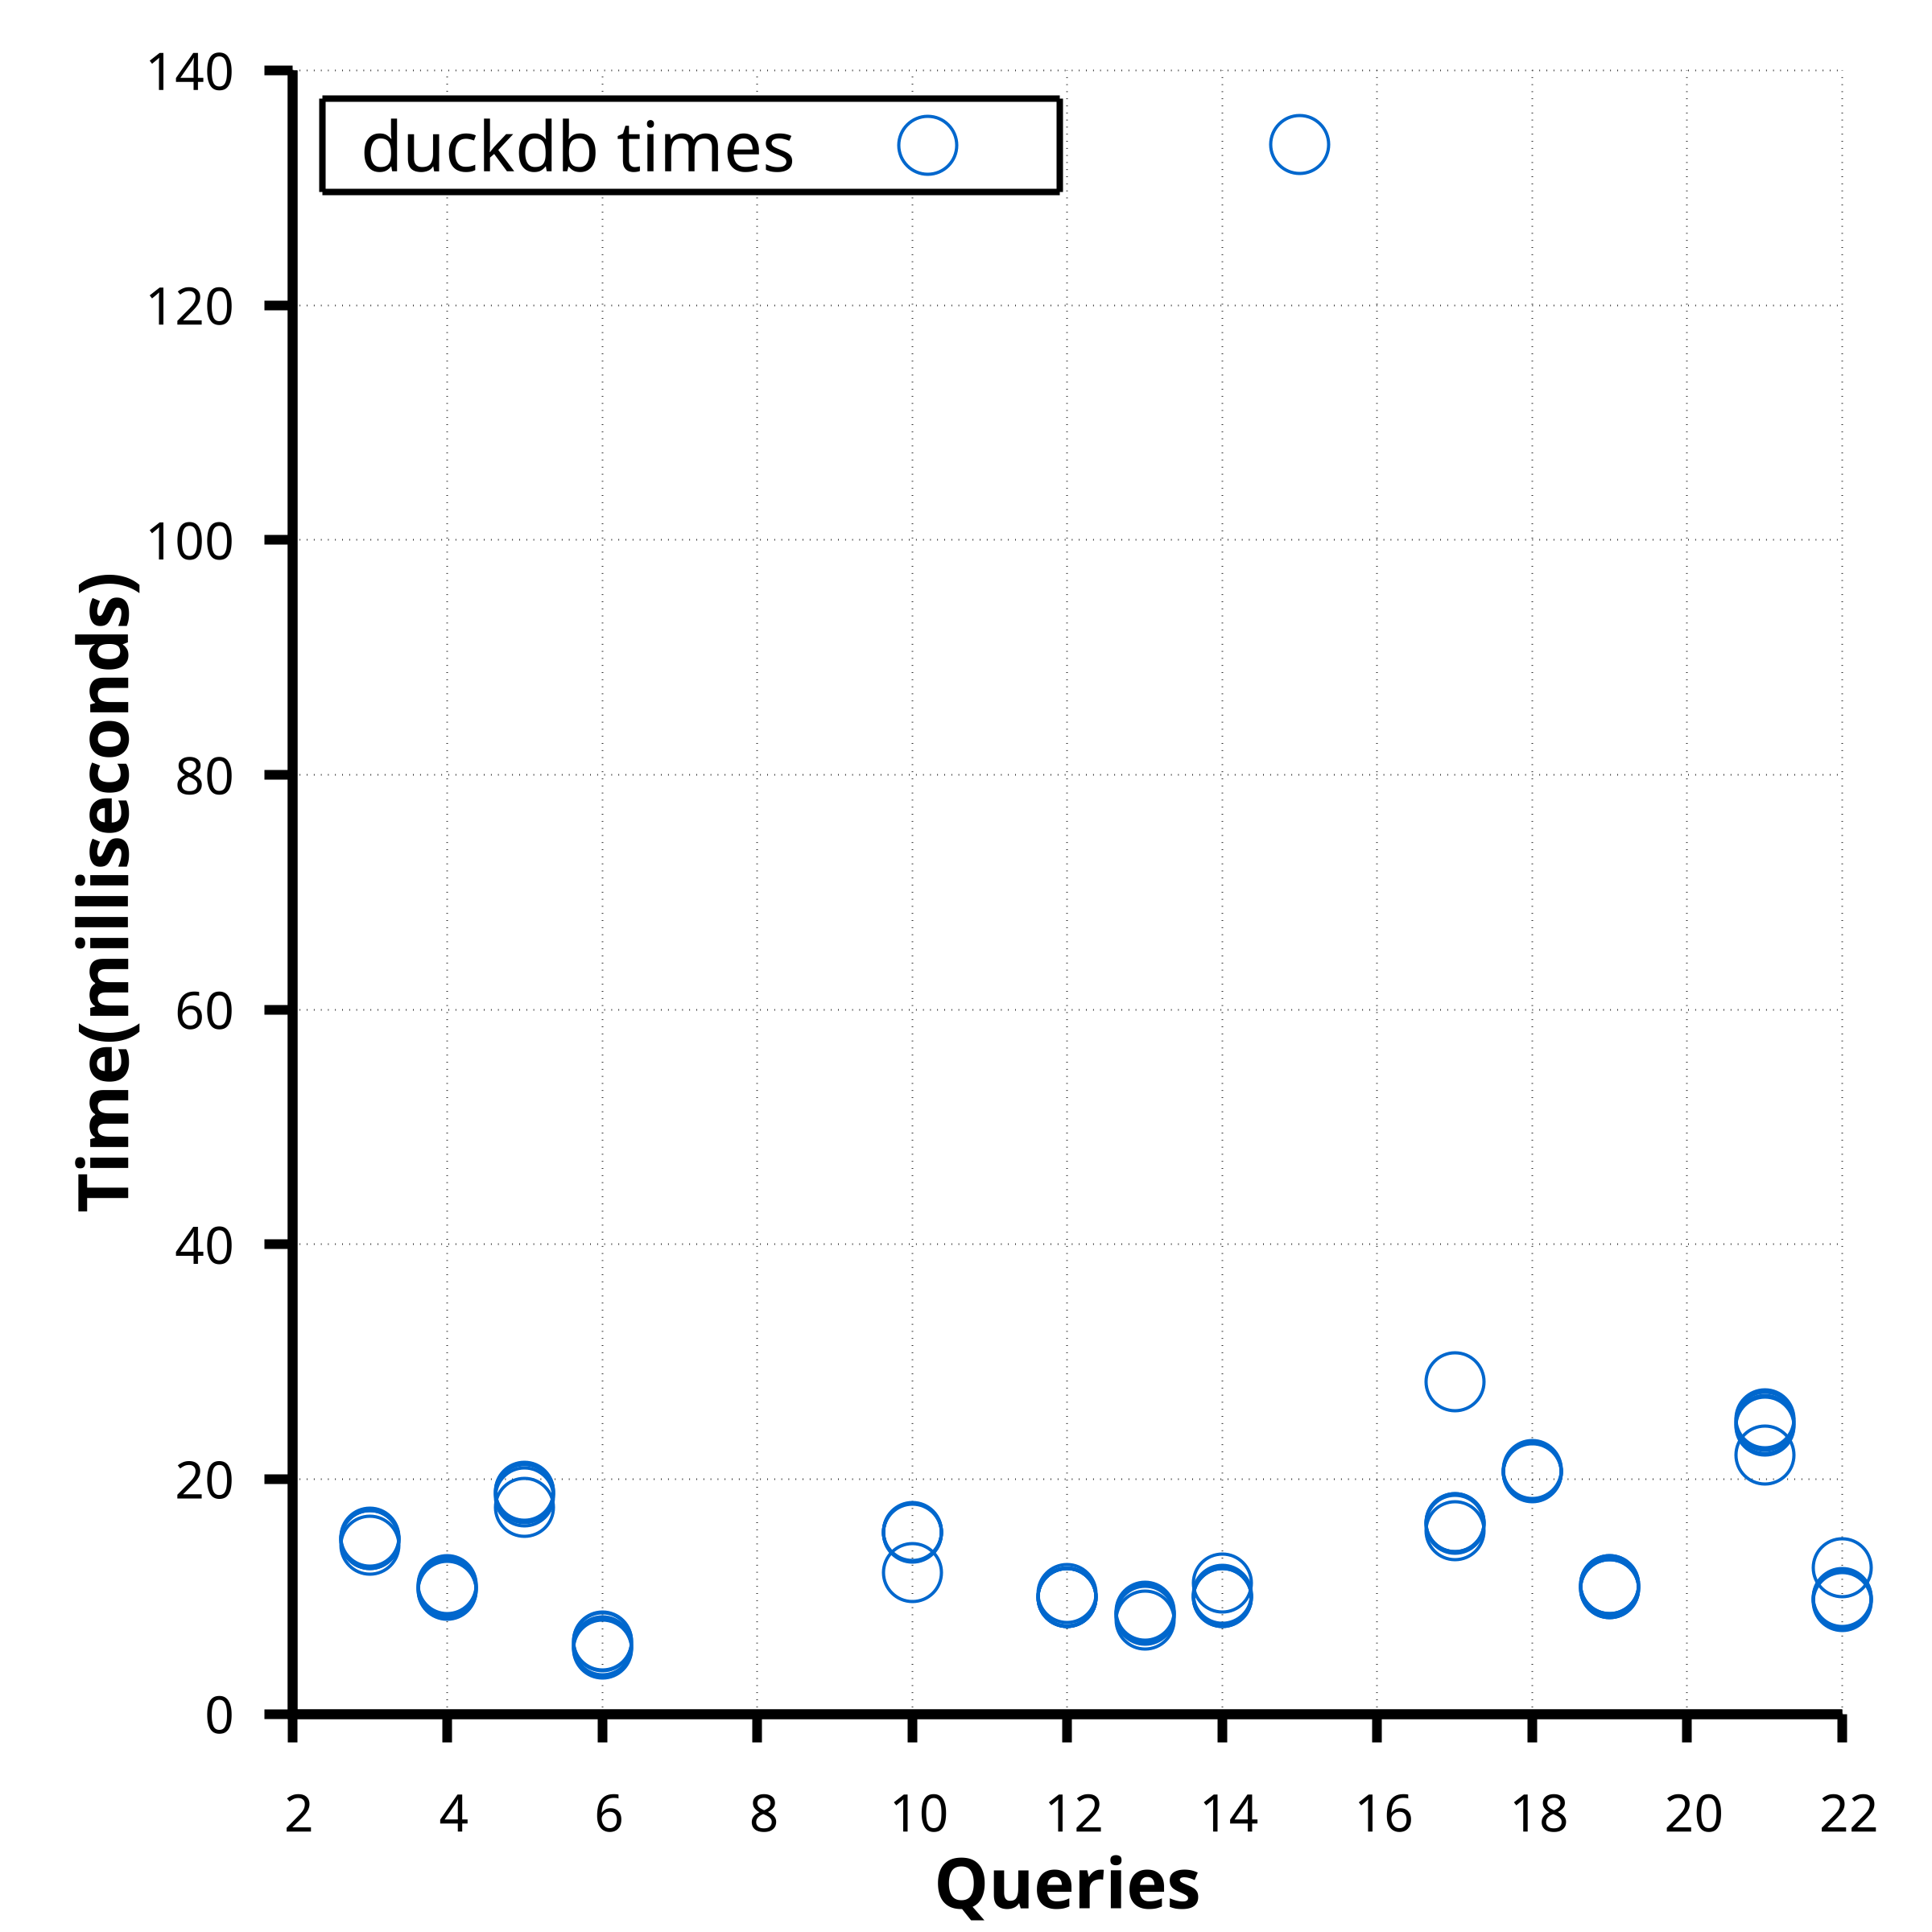
\includegraphics[width=\textwidth]{duckdb.png}
      \caption{DuckDB execution times}
      \label{fig:duckdb_times}
    \end{subfigure}
    \hfill
    \begin{subfigure}[b]{0.48\textwidth}
      \centering
      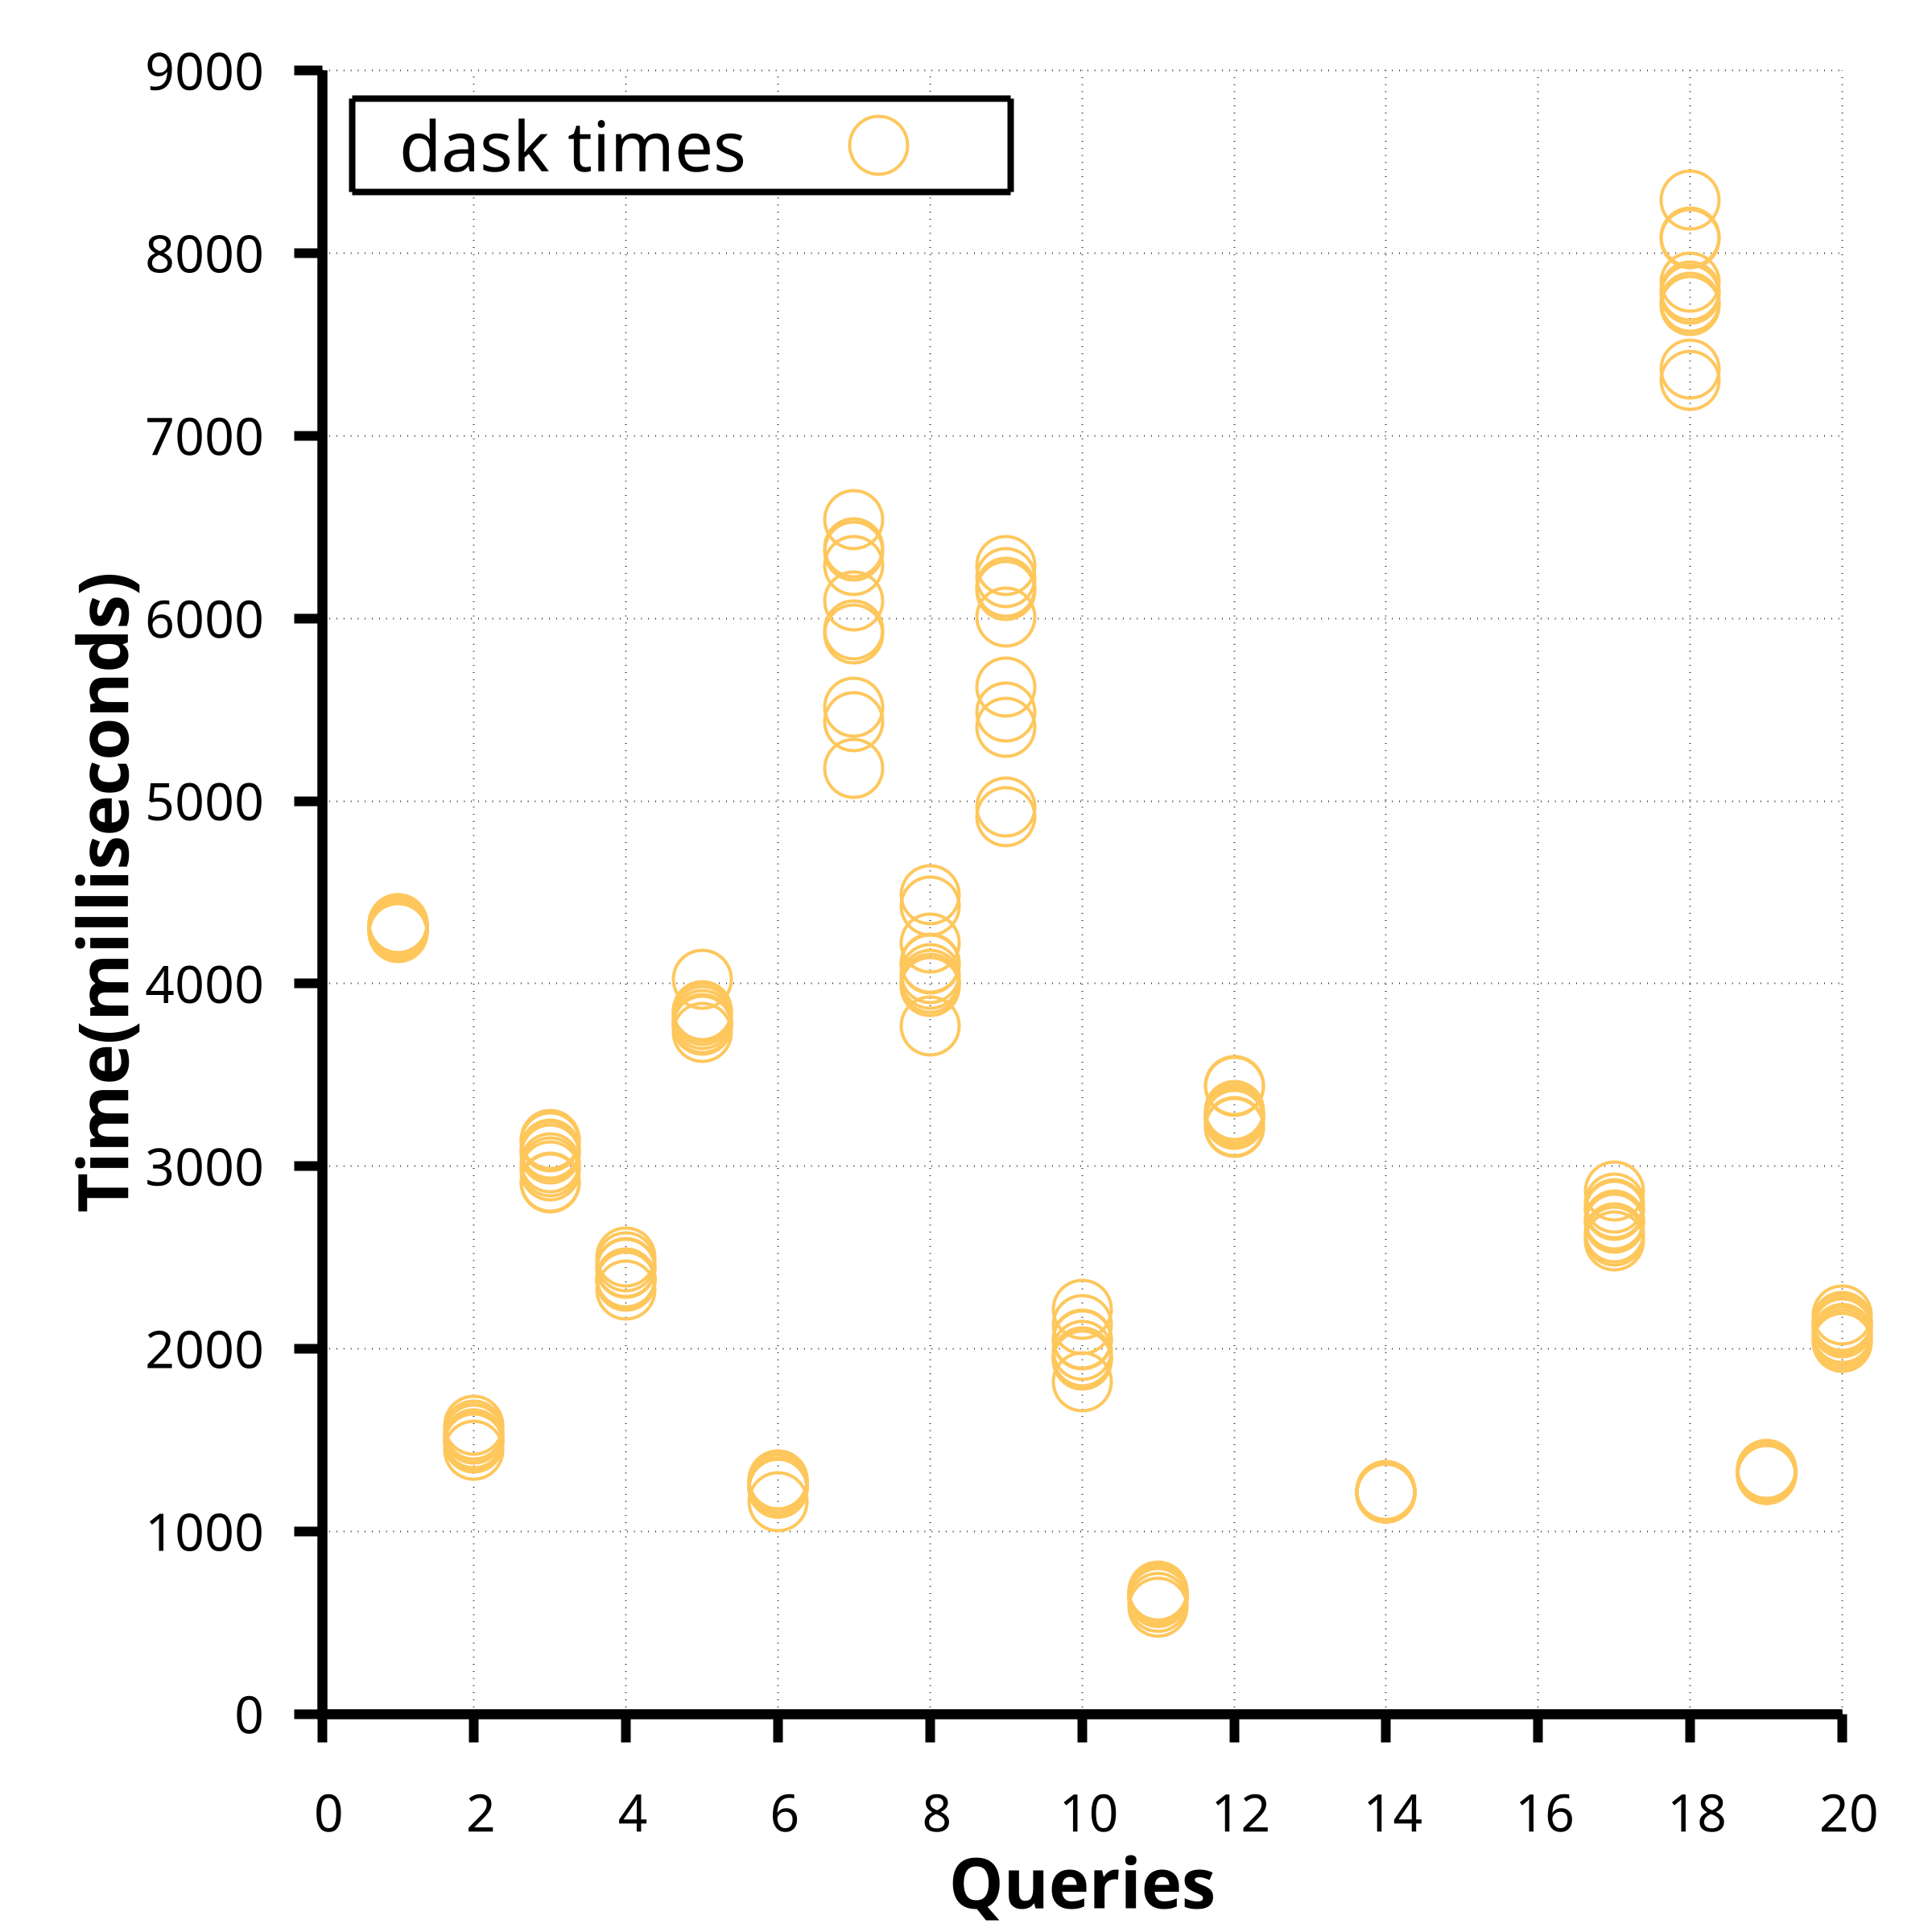
\includegraphics[width=\textwidth]{dask.png}
      \caption{Dask SQL execution times}
      \label{fig:dask_times}
    \end{subfigure}
    \begin{subfigure}[b]{0.6\textwidth}
      \centering
      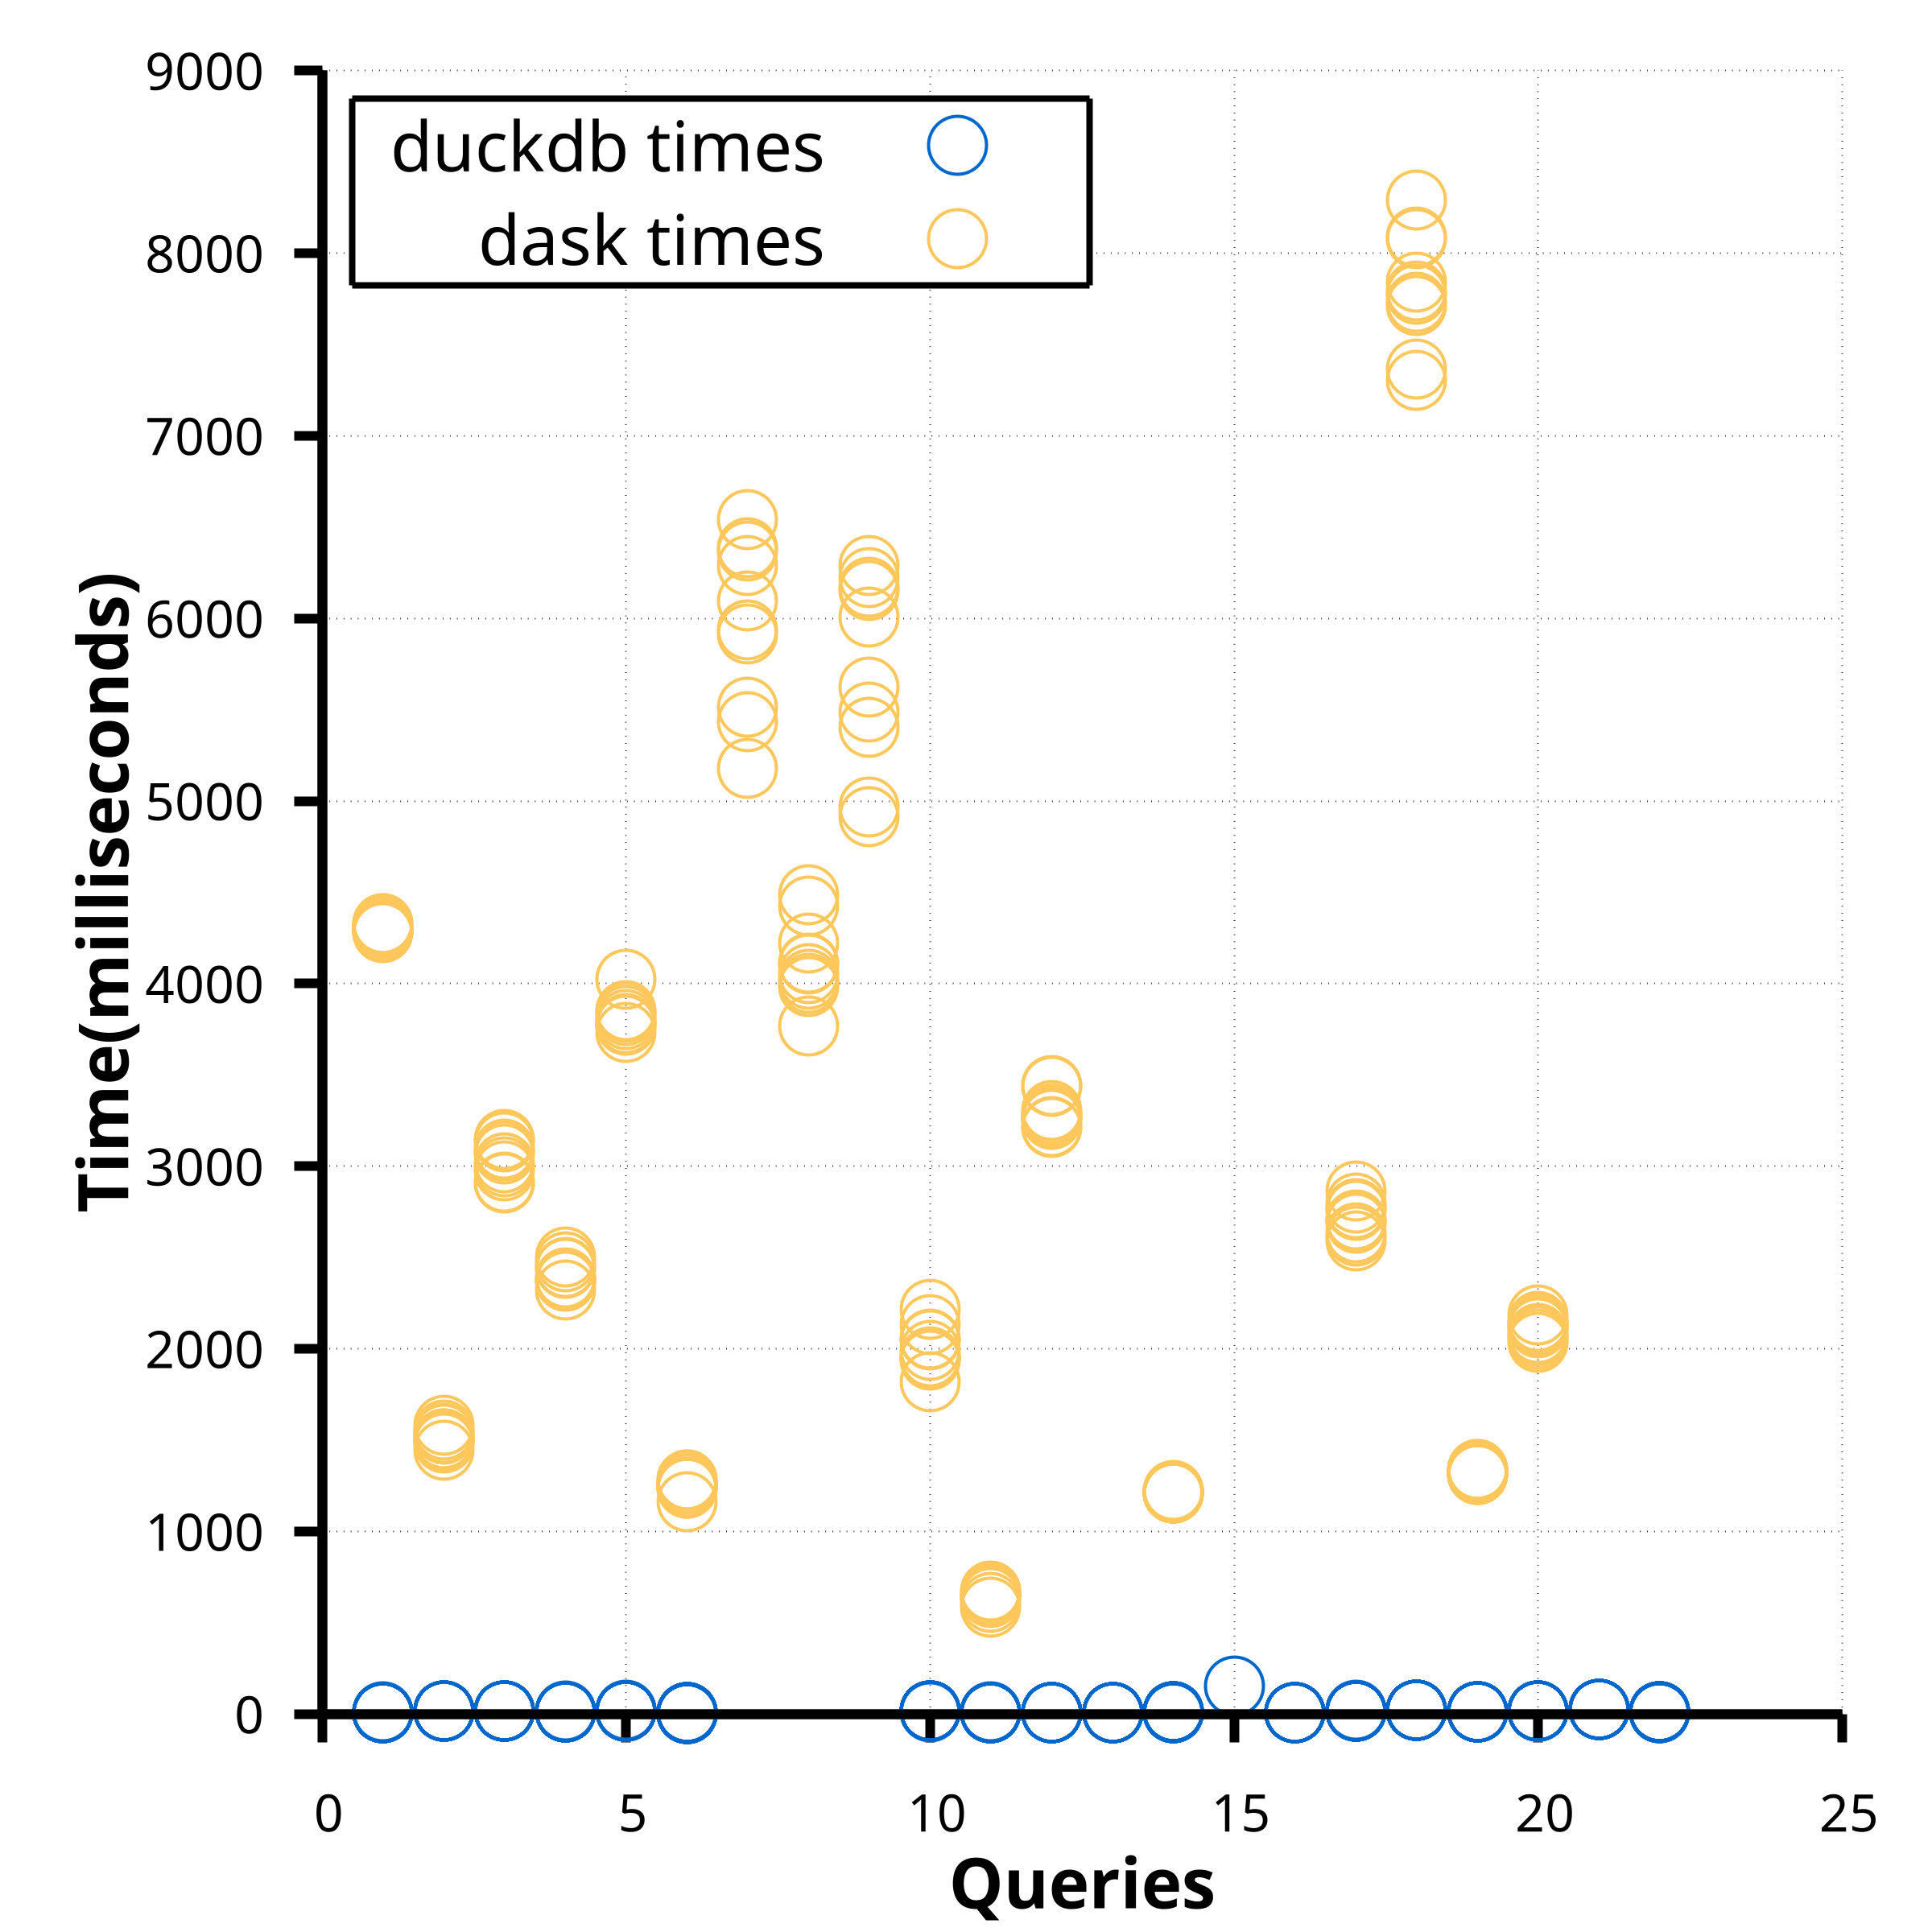
\includegraphics[width=\textwidth]{merge.png}
      \caption{Comparing DuckDB and Dask SQL execution times}
      \label{fig:comparing_times}
    \end{subfigure}
  \end{figure}

  Como se puede ver en la figura \ref{fig:duckdb_times} y \ref{fig:dask_times}
  se puede ver que los tiempos de ejecución de \ti{DuckDB} son menores que los
  tiempos de ejecución de \ti{Dask SQL}, esto se debe quizá al tamaño del dataset
  propuesto.
